\setcounter{section}{6}
\section{How to Draw Monoidal Categories}

\setcounter{subsection}{1}
\subsection{Planar Diagrams for 2-Categories}

\begin{exercise}[2.7.2.8]\label{ex:2.7.2.8}
  Show that the axioms of a 2-category imply the following equalities.
  \begin{equation}\label{eq:2.7.2.8:1}
    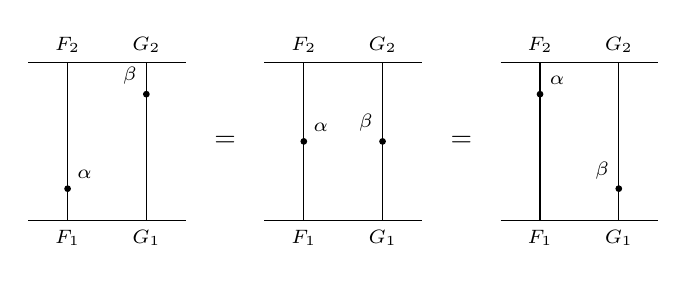
\begin{tikzpicture}[baseline]
      \draw (-1,1) -- (1,1);

      \coordinate (F2) at (-0.5, 1);
      \coordinate (F1) at (-0.5, -1);
      \coordinate (G2) at (0.5, 1);
      \coordinate (G1) at (0.5, -1);

      \coordinate (E) at (-0.7, 0);
      \coordinate (D) at (0, 0);
      \coordinate (C) at (0.7, 0);

      \node at (E) {$\EE$};
      \node at (D) {$\DD$};
      \node at (C) {$\CC$};

      \draw (F2) node[font=\scriptsize,above] {$F_2$} -- (F1) node[font=\scriptsize,below] {$F_1$};
      \draw (G2) node[font=\scriptsize,above] {$G_2$} -- (G1) node[font=\scriptsize,below] {$G_1$};

      \coordinate (a) at (-0.5, -0.6);
      \coordinate (b) at (0.5, 0.6);

      \draw[fill=black] (a) circle (1pt) node[font=\scriptsize,anchor=south west] {$\alpha$};
      \draw[fill=black] (b) circle (1pt) node[font=\scriptsize,anchor=south east] {$\beta$};

      \draw (-1,-1) -- (1,-1);

      \node at (1.5, 0) {$=$};

      \begin{scope}[xshift=3cm]
        \draw (-1,1) -- (1,1);

        \coordinate (F2) at (-0.5, 1);
        \coordinate (F1) at (-0.5, -1);
        \coordinate (G2) at (0.5, 1);
        \coordinate (G1) at (0.5, -1);

        \coordinate (E) at (-0.7, 0);
        \coordinate (D) at (0, 0);
        \coordinate (C) at (0.7, 0);

        \node at (E) {$\EE$};
        \node at (D) {$\DD$};
        \node at (C) {$\CC$};

        \draw (F2) node[font=\scriptsize,above] {$F_2$} -- (F1) node[font=\scriptsize,below] {$F_1$};
        \draw (G2) node[font=\scriptsize,above] {$G_2$} -- (G1) node[font=\scriptsize,below] {$G_1$};

        \coordinate (a) at (-0.5, 0);
        \coordinate (b) at (0.5, 0);

        \draw[fill=black] (a) circle (1pt) node[font=\scriptsize,anchor=south west] {$\alpha$};
        \draw[fill=black] (b) circle (1pt) node[font=\scriptsize,anchor=south east] {$\beta$};

        \draw (-1,-1) -- (1,-1);
      \end{scope}

      \node at (4.5, 0) {$=$};

      \begin{scope}[xshift=6cm]
        \draw (-1,1) -- (1,1);

        \coordinate (F2) at (-0.5, 1);
        \coordinate (F1) at (-0.5, -1);
        \coordinate (G2) at (0.5, 1);
        \coordinate (G1) at (0.5, -1);

        \coordinate (E) at (-0.7, 0);
        \coordinate (D) at (0, 0);
        \coordinate (C) at (0.7, 0);

        \node at (E) {$\EE$};
        \node at (D) {$\DD$};
        \node at (C) {$\CC$};

        \draw (F2) node[font=\scriptsize,above] {$F_2$} -- (F1) node[font=\scriptsize,below] {$F_1$};
        \draw (G2) node[font=\scriptsize,above] {$G_2$} -- (G1) node[font=\scriptsize,below] {$G_1$};

        \coordinate (a) at (-0.5, 0.6);
        \coordinate (b) at (0.5, -0.6);

        \draw[fill=black] (a) circle (1pt) node[font=\scriptsize,anchor=south west] {$\alpha$};
        \draw[fill=black] (b) circle (1pt) node[font=\scriptsize,anchor=south east] {$\beta$};

        \draw (-1,-1) -- (1,-1);
      \end{scope}
    \end{tikzpicture}
  \end{equation}
  \begin{equation}\label{eq:2.7.2.8:2}
    \begin{tikzpicture}[baseline]
      \draw (-1,1) -- (1,1);

      \coordinate (F2) at (-0.5, 0.6);
      \coordinate (F1) at (-0.5, -1);
      \coordinate (G2) at (0.5, 1);
      \coordinate (G1) at (0.5, -0.6);

      \coordinate (C1) at (-0.7, 0);
      \coordinate (C2) at (0.7, 0);

      \node at (C1) {$\CC$};
      \node at (C2) {$\CC$};

      \draw (F2) -- (F1) node[font=\scriptsize,below] {$F_1$};
      \draw (G2) node[font=\scriptsize,above] {$G_2$} -- (G1);

      \draw[fill=black] (F2) circle (1pt) node[font=\scriptsize,anchor=south west] {$\alpha$};
      \draw[fill=black] (G1) circle (1pt) node[font=\scriptsize,anchor=south east] {$\beta$};

      \draw (-1,-1) -- (1,-1);

      \node at (1.5, 0) {$=$};

      \begin{scope}[xshift=3cm]
        \draw (-1,1) -- (1,1);

        \coordinate (F2) at (0, -0.4);
        \coordinate (F1) at (0, -1);
        \coordinate (G1) at (0, 0.4);
        \coordinate (G2) at (0, 1);

        \coordinate (C1) at (-0.7, 0);
        \coordinate (C2) at (0.7, 0);

        \node at (C1) {$\CC$};
        \node at (C2) {$\CC$};

        \draw (F2) -- (F1) node[font=\scriptsize,below] {$F_1$};
        \draw (G2) node[font=\scriptsize,above] {$G_2$} -- (G1);

        \draw[fill=black] (F2) circle (1pt) node[font=\scriptsize,anchor=south west] {$\alpha$};
        \draw[fill=black] (G1) circle (1pt) node[font=\scriptsize,anchor=south east] {$\beta$};

        \draw (-1,-1) -- (1,-1);

        \node at (1.5, 0) {$=$};
      \end{scope}

      \node at (4.5, 0) {$=$};

      \begin{scope}[xshift=6cm]
        \draw (-1,1) -- (1,1);

        \coordinate (F2) at (0.4, 0.6);
        \coordinate (F1) at (0.4, -1);
        \coordinate (G2) at (-0.4, 1);
        \coordinate (G1) at (-0.4, -0.6);

        \coordinate (C1) at (-0.7, 0);
        \coordinate (C2) at (0.7, 0);

        \node at (C1) {$\CC$};
        \node at (C2) {$\CC$};

        \draw (F2) -- (F1) node[font=\scriptsize,below] {$F_1$};
        \draw (G2) node[font=\scriptsize,above] {$G_2$} -- (G1);

        \draw[fill=black] (F2) circle (1pt) node[font=\scriptsize,anchor=south west] {$\alpha$};
        \draw[fill=black] (G1) circle (1pt) node[font=\scriptsize,anchor=south east] {$\beta$};

        \draw (-1,-1) -- (1,-1);
      \end{scope}
    \end{tikzpicture}
  \end{equation}
\end{exercise}

\begin{solution}[2.7.2.8]\label{sol:7.8}
  The diagram \ref{eq:2.7.2.8:1} follows from the axioms of a 2-category. In particular, the interchange law states that horizontal and vertical compositions of 2-morphisms are compatible. More precisely, given 2-morphisms $\alpha: F_1 \implies F_2$ and $\beta: G_1 \implies G_2$, the horizontal composition $\beta \ast \alpha : G_1 \circ F_1 \implies G_2 \circ F_2$ is defined, and satisfies:
  \[%
    (\beta' \circ \beta) \ast (\alpha' \circ \alpha) = (\beta' \ast \alpha') \circ (\beta \ast \alpha)
  .\]%
  In \ref{eq:2.7.2.8:1}, each equality reflects this interchange identity. That is, we may either first compose vertically and then horizontally, or compose horizontally first and then vertically, and the result is the same. This coherence condition is one of the core structural axioms of any strict 2-category.

  For diagram \ref{eq:2.7.2.8:2}, this identity expresses the fact that the horizontal composition of 2-morphisms with identity 1-morphisms on either side is strictly associative, and that such composition is natural. Specifically, suppose:
  \[%
    \alpha: F_1 \implies G_2 \aand \beta: \mathrm{id}_\CC \implies \mathrm{id}_\CC
  ,\]%
  are 2-morphisms in the hom-category $\CC(\CC, \CC)$. Then, under horizontal composition, we form:
  \[%
    (\mathrm{id}_{\CC} \ast \alpha) \circ (\beta \ast \mathrm{id}_{F_1}) = (\beta \circ \mathrm{id}_{\CC}) \ast (\mathrm{id}_{\CC} \circ \alpha) = \beta \ast \alpha
  .\]%

  This follows from the interchange law and the unit laws of 2-categories. In particular, composing with identity 2-morphisms has no effect, and the strict associativity of composition allows us to freely rebracket the diagram. This justifies the equality of all three diagrams above.
\end{solution}

\setcounter{subsection}{3}
\subsection{The Temperley–Lieb Category}

\begin{exercise}[2.7.4.16]\label{ex:2.7.4.16}
  We can view the algebra $A = \R[x]/(x^2)$ as an object in the monoidal category of $\R$-vector spaces. Let $\Cap : A \otimes A \to \R$ denote the linear map which sends $f \otimes g$ to the coefficient of $x$ in $fg$. Let $\Cup : \R \to A \otimes A$ denote the map which sends $1$ to $x \otimes 1 + 1 \otimes x$.

  \begin{enumerate}
    \item We wish to encode these maps diagrammatically, drawing $\Cap$ as a cap and $\Cup$ as a cup. Justify this diagrammatic notation, by checking the isotopy relations.

    \item Draw a sequence of nested circles, as in an archery target. Evaluate this morphism.
  \end{enumerate}
\end{exercise}

\begin{solution}[2.7.4.16(i)]\label{sol:2.7.4.16i}
  Let $v = ax + b \in A$. To check isotopy relations, we need to check the following compositions: $(\cap \otimes \id_A) \circ (\id_A \otimes \Cup)(ax + b)$ and $(\id_A \otimes \Cup) \circ (\cap \otimes \id_A)(ax + b)$. To keep notation simple, recall that $\R \otimes A \cong A \cong A \otimes \R$.

  We deal with the first composition first. We know that $\id_A \otimes \Cup : A \to A \otimes A \otimes A$, we get
  \[%
    (\id_A \otimes \Cup)(ax + b) = (ax + b) \otimes (x \otimes 1 + 1 \otimes x) = (ax + b) \otimes x \otimes 1 + (ax + b) \otimes 1 \otimes x
  .\]%
  Now, we know that $\Cap \otimes \id_A : A \otimes A \otimes A \to A$, applying this to the above, we get
  \[%
    (\Cap \otimes \id_A) \circ (\id_A \otimes \Cup)(ax + b) = (\Cap \otimes \id_A)((ax + b) \otimes x \otimes 1 + (ax + b) \otimes 1 \otimes x)
  .\]%
  Computing $\Cap((ax + b) \otimes x)$, we compute $fg$ to get $(ax + b) \cdot x = ax^2 + bx$. Therefore, $\Cap((ax + b) \otimes x) = b$. Similarly, we get $\Cap((ax + b) \otimes 1) = a$. Therefore, we have
  \[%
    (\Cap \otimes \id_A) \circ (\id_A \otimes \Cup)(ax + b) = b + ax = ax + b
  .\]%
  Therefore, we have shown that the first composition is the identity.

  We now deal with the second composition, $(\id_A \otimes \Cup) \circ (\cap \otimes \id_A)(ax + b)$. Computing the inner composition, $\Cup \otimes \id_A : A \otimes A \to A \otimes A \otimes A$, we get
  \[%
    (\Cup \otimes \id_A)(ax + b) = (x \otimes 1 + 1 \otimes x) \otimes (ax + b) = x \otimes 1 \otimes (ax + b) + 1 \otimes x \otimes (ax + b)
  .\]%
  Now, we know that $\id_A \otimes \Cap : A \otimes A \otimes A \to A$, so applying this to the above, we get
  \[%
    (\id_A \otimes \Cap)(x \otimes 1 \otimes (ax + b) + 1 \otimes x \otimes (ax + b)) = ax + b
  .\]%
  Therefore, $(\id_A \otimes \Cap) \circ (\Cup \otimes \id_A)(ax + b) = ax + b$, as desired.

  Thus, we have shown that the isotopy relations hold in vector spaces.
\end{solution}

\begin{solution}[2.7.4.16(ii)]\label{sol:2.7.4.16ii}
  Let $f$ be the entire morphism. For simplicity, I use the notation, $\Cup^{\otimes k} : \R \to A^{\otimes k}$, $\Cap^{\otimes k} : A^{\otimes k} \to \R$, and $f^k = \Cap^{\otimes k} \circ \Cup^{\otimes k} : \R \to \R$, to denote $k$-circles.

  For the $1$-circle case, we have the following morphism
  \[%
    f(1) = (\Cap \circ \Cup)(1) = \Cap(\Cup(1)) = \Cap(x \otimes 1 + 1 \otimes x) = 1 + 1 = 2
  .\]%
  For the $2$-circle case, we have the following morphism
  \[%
    f^2(1) = \left(\cap^{\otimes 2} \circ \cup^{\otimes 2}\right)(1) = \cap^{\otimes 2}\left(\cup^{\otimes 2}(1)\right) = \cap^{\otimes 2}(x \otimes 1 + 1 \otimes x \otimes x \otimes 1 + 1 \otimes x) = 4
  .\]%
  For the $k$-circle case, we have the following morphism
  \[%
    f^k(1) = \left(\cap^{\otimes k} \circ \cup^{\otimes k}\right)(1)
  .\]%
  Since $\Cup(1) = x \otimes 1 + 1 \otimes x$, then $\Cup^{\otimes k}(1)$ is the sum of $2^k$ simple tensors, each term of the form $v_1 \otimes w_1 \otimes \cdots \otimes v_k \otimes w_k$, where each pair $(v_i \otimes w_i)$ is either $x \otimes 1$ or $1 \otimes x$. Applying $\Cap^{\otimes k}$ to each such term gives $1$ for every pair, since $\Cap(x \otimes 1) = \Cap(1 \otimes x) = 1$. Therefore, we get $f^k(1) = 2^k$.
\end{solution}

\begin{exercise}[2.7.4.17]\label{ex:7.17}
  This question is about the Temperley–Lieb category.
  \begin{enumerate}
    \item Finish the proof that the isotopy relation holds in vector spaces.

    \item There is a map $V \otimes V \to V \otimes V$ which sends $x \otimes y \mapsto y \otimes x$. Draw this as an element of the Temperley–Lieb category (a linear combination of diagrams).

    \item Find an endomorphism of $2$ strands which is killed by placing a cap on top. Can you find one which is an idempotent? Also find an endomorphism killed by putting a cup on bottom.

    \item (Harder) Find an idempotent endomorphism of $3$ strands which is killed by a cap on top (for either of the two placements of the cap). \end{enumerate}
\end{exercise}

\begin{solution}[2.7.4.17(i)]\label{sol:7.17i}
  Define the following swap function:
  \[%
    \tau^k\left(\bigotimes_{n=1}^k v_n\right) = \bigotimes_{n=1}^k v_{k-n+1}
  .\]%
  I'll be using the notation $\left\lfloor f^k(x) \right\rfloor$ to denote the coefficient of $x^k$ in the polynomial $f(x)$.

  To prove isotopy relations hold in vector spaces, we need to prove the following:
  the following identities,
  \begin{align*}
    (\Cap \otimes \id_V) \circ (\id_V \otimes \Cup) &= \id_V \\
    (\id_V \otimes \Cap) \circ (\Cup \otimes \id_V) &= \id_V
  ,\end{align*}
  loop evaluation, symmetry of cups and caps, and sliding. I've already shown the snake identities in \ref{sol:2.7.4.16i} and the loop evaluation in \ref{sol:2.7.4.16ii}.
\end{solution}

\begin{solution}[2.7.4.17(ii)]\label{sol:7.17ii}
\end{solution}

\begin{solution}[2.7.4.17(iii)]\label{sol:7.17iii}
\end{solution}

\subsection{More About Isotopy}

\begin{exercise}[2.7.5.19]\label{ex:7.19}
  One can think about the right mate and the left mate as ``twisting'' or ``rotating'' $\alpha$ by $180^{\circ}$ to the right or to the left. Visualize what it would mean to twist $\alpha$ by $360^{\circ}$ to the right, yielding another $2$-morphism $\alpha^{\vee\vee} : E \to F$. Verify that $^\vee\alpha = \alpha^\vee$, if and only if $\alpha = \alpha^{\vee\vee}$. Thus cyclicity is the same as ``$360$ degree rotation invariance,'' which one might expect from any planar picture.
\end{exercise}

\begin{solution}[2.7.5.19]\label{sol:7.19}
\end{solution}

\begin{exercise}[2.7.5.20]\label{ex:7.20}
  Suppose that $B$ is an object in a monoidal category with biadjoints, and $\Phi : B \otimes B \otimes B \to \mathbb{1}$ is a cyclic morphism. What should it mean to ``rotate'' $\Phi$ by $120^{\circ}$? Suppose that $\Hom(B \otimes B \otimes B, \mathbb{1})$ is one-dimensional over $\C$. What can you say about the $120^{\circ}$ rotation of $\Phi$, vis a vis $\Phi$? What if $\Hom(B \otimes B \otimes B, \mathbb{1})$ is one-dimensional over $\R$?
\end{exercise}

\begin{solution}[2.7.5.20]\label{sol:7.20}
\end{solution}
